%!TEX root = .../tfg_im.tex

\chapter{Desarrollo}

\section{Descripción}

\subsection{Funciones del sistema}

\displayquote{``La aplicación que se va a desarrollar tiene como objetivo recoger información de las diferentes redes sociales, almacenarlos en una base de datos y mostrarlos en nuestro sitio web. Esos datos almacenados,son una fuente de información fiable que nos permite conocer que se esta concinando en el mundo en este momento. Para ello se deberá tener en cuenta la gestión de:''}


\vspace{5 mm}

\begin{itemize}

\item Control de Acceso: En la aplicación existirán 3 tipos de roles:

\begin{itemize}
\item Administrador: Tendrá el control de gestionar la información proveniente de las API's.El Filtrado de los datos o la frecuencia con la que realiza las peticiones la aplicación con las API's.
También podrá gestionar el contenido del sistema
\item Colaborador: Podrá publicar contenido en la aplicación.
\item Usuario no registrado: Tendrá acceso a la visualización de los datos de la aplicación. 
\end{itemize}

\end{itemize}

\section{Análisis}


\subsection{Tweet}

\subsection{API de Twitter}

\subsection{Google Maps}

\subsection{API de Google}


\section{Especificación de Requisitos}

Para este apartado se ha seguido el estándar IEEE 830 de especificación de requisitos.

\subsection{Requisitos funcionales}

Para ordenar los requisitos funcionales, se ha considerado que la forma más adecuada es por tipo de rol y relevancia. Los identificadores de los requisitos que pertenezcan al rol de administrador empezarán por A, los que pertenezcan al rol de usuario empezarán por U, los que pertenezcan al sistema empezarán por S. Para ordenar por relevancia, se especificán tres casos: Los requisitos que sean funcionalidades básicas de la aplicación empezarán por FB, los requisitos que sean funcionalidades secundarias empezarán FS.


%Requisito 1
\begin{table}[h!]
\centering
\begin{tabular}{|p{3cm}|p{10cm}|}
\hline
Identificador & FB-U-01 \\ \hline
Actor involucrado & Usuario \\ \hline
Nombre & Ver listado de entradas \\ \hline
Descripción & Desde la página de blog o un buscador se podrá acceder a ver un listado de las entradas del blog. Cada elemento del listado contendrá una foto de la entrada, un titulo y un resumen \\ \hline
Requisitos lógicos & Podrán existir una serie de datos generados por usuarios,como comentarios. \\ \hline
\end{tabular}
\end{table}


%Requisito 2
\begin{table}[h!]
\centering
\begin{tabular}{|p{3cm}|p{10cm}|}
\hline
Identificador & FB-U-02 \\ \hline
Actor involucrado & Usuario \\ \hline
Nombre & Ver detalle de entrada \\ \hline
Descripción & En el detalle de la entrada,  \\ \hline
Requisitos lógicos & La información estará normalizada, existiendo una serie de datos comunes a todas las entradas, pero podrán existir ciertos datos adicionales según el tipo de entrada. También podrán existir una serie de datos generados por usuarios, como valoraciones y comentarios. \\ \hline
\end{tabular}
\end{table}


%Requisito 3
\begin{table}[h!]
\centering
\begin{tabular}{|p{3cm}|p{10cm}|}
\hline
Identificador & FB-U-03 \\ \hline
Actor involucrado & Usuario \\ \hline
Nombre & Comentar Entrada\\ \hline
Descripción & En el detalle de la entrada,  \\ \hline
Requisitos lógicos & La información estará normalizada, existiendo una serie de datos comunes a todas las entradas, pero podrán existir ciertos datos adicionales según el tipo de entrada. También podrán existir una serie de datos generados por usuarios, como valoraciones y comentarios. \\ \hline
\end{tabular}
\end{table}

%Requisito 4
\begin{table}[h!]
\centering
\begin{tabular}{|p{3cm}|p{10cm}|}
\hline
Identificador & FB-U-03 \\ \hline
Actor involucrado & Usuario \\ \hline
Nombre & Ver listado de tweets\\ \hline
Descripción & En el mapa de la aplicación se geoposicionarán los tweets  \\ \hline
Requisitos lógicos & Los tweets \\ \hline
\end{tabular}
\end{table}


%Requisito 4
\begin{table}[h!]
\centering
\begin{tabular}{|p{3cm}|p{10cm}|}
\hline
Identificador & FB-U-04 \\ \hline
Actor involucrado & Usuario \\ \hline
Nombre & Filtrar listado de tweets\\ \hline
Descripción & En el detalle de la entrada,  \\ \hline
Requisitos lógicos & La información estará normalizada, existiendo una serie de datos comunes a todas las entradas, pero podrán existir ciertos datos adicionales según el tipo de entrada. También podrán existir una serie de datos generados por usuarios, como valoraciones y comentarios. \\ \hline
\end{tabular}
\end{table}


\section{Casos de Uso}

\begin{landscape}
\begin{figure}
\begin{center}
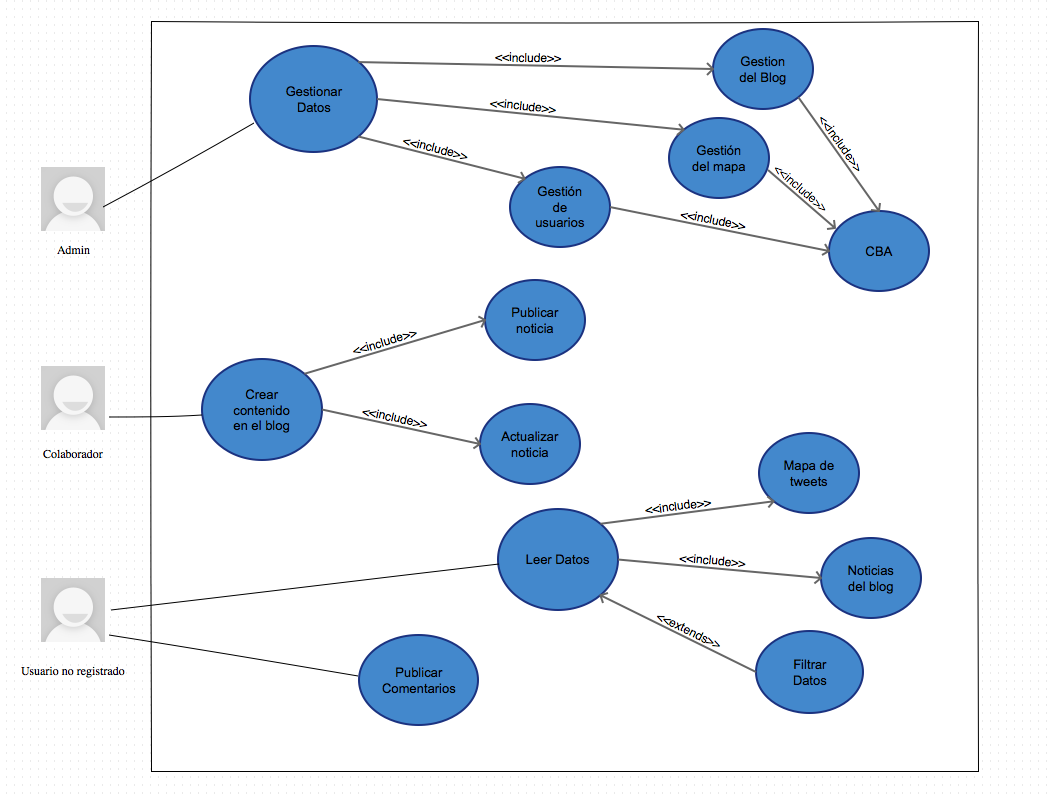
\includegraphics[width=16cm]{imagenes/casos-de-uso.png}
\caption{Casos de uso}
\label{casos_uso}
\end{center}
\end{figure}
\end{landscape}

Para mostrar las actividades se utilizará una representación mediante casos de uso. Los casos de uso se han segmentado para cada rol de la aplicación. En la figura \ref{casos_uso}  se representan los casos de uso para cada rol que se explicarán a continuación:

\vspace{5 mm}

El \textbf{usuario no registrado}, es el rol por defecto en la aplicación cuando el usuario no tiene ninguna acreditación en la web y carece de permisos. El usuario no registrado podrá solicitar los datos de la aplicación para visualizar el contenido. Por ejemplo podrá solicitar los datos del mapa de tweets o del blog. Tambíen podrá filtrar la información de los datos solicitados, por palabras clave o categorías. Este usuario podrá también publicar comentarios en el blog.

\vspace{5 mm}

El \textbf{colaborador}, este rol, además de poder realizar las mismas funciones que el usuario no registrado, tiene unos permisos añadidos. Este usuario tiene la función extra de publicar contenido en el blog. Un usuario colaborador, podrá crear noticias que luego aparecerán en el blog. Podrá actualizar las noticias, pero únicamente aquellas que hayan sido creadas por él. No tendrá permisos para borrar contenido del blog.

\vspace{5 mm}

Por último esta el \textbf{administrador}, el rol de administrador, es el de superusuario, ya que posee todos los permisos. El administrador es el encargado de gestionar todo el contenido de la web. Dentro del contenido se encuentran los tres principales modelos de datos. El primer modelo de datos son los \textquote{Tweets}, el administrador se encargará de gestionar la frecuencia con la que se actualiza el mapa de tweets, para tener representada la información actualizada. Otra función será modificar la recolección de tweets en base a una palabra clave, que el administrador introducirá manualmente. El siguiente modelo son las noticias, el administrador podrá generar contenido en el blog, creando o borrando cualquier tipo de contenido, tanto propio como de un colaborador. El administrador también podrá moderar los comentarios de las entradas del blog. Por último el último el último modelo de datos serían los usuarios. El administrador gestionará los datos de los usuarios de la aplicación, siendo el encargado tanto de dar de alta a los colaboradores generando un usuario y contraseña como darlos de baja. Toda la gestión del contenido implica crear,borrar o actualizar información de forma que se ha representado mediante un caso de uso: CBA.


\section{Diseño de Arquitectura}

\subsection{Arquitectura MVC}

La rama de la ingenieria del software se preocupa por crear productos robustos y de calidad. Una de las principales soluciones para conseguir esos objetivos, es la arquitectura basada en capas, que separa el código en función de sus responsabilidades.Una de las arquitecturas más populares basada en capas para el desarrollo de aplicaciones web, es la arquitectura MVC(Modelo-Vista-Controlador). Mediante esta arquitectura se divide el sistema en tres capas:

\begin{itemize}

\item \textbf{El Modelo}: Capa que trabaja con los datos, contiene mecanismos para acceder a la información. A través del modelo accederemos a la base de datos donde estarán los datos.
\item \textbf{El Controlador}: Responde generalmente a acciones del usuario, e invoca esas peticiones al modelo, como por ejemplo un registro en una base de datos. También responde al envío de datos a la vista.
\item \textbf{La Vista}: Es la capa encargada de presentar la información de nuestra página. El código que nos permitirá renderizar los estados de nuestra aplicación en HTML.

\end{itemize}

\vspace{5 mm}

El diagrama de la figura \ref{logo_mvc} muestra los modos de colaboración de las diferentes capas de una aplicación MVC. Incialmente el usuario realiza una solicitud a la aplicación web, y esta le llega al controlador. El controlador que se comunica tanto con el modelo como con la vista, le solicita los datos al modelo o manda actualizaciones de los datos y una vez realizadas las operaciones pertinentes le solicita la salida de los datos a la vista. Por último las vistas envían al usuario la salida.


\begin{figure}
\begin{center}
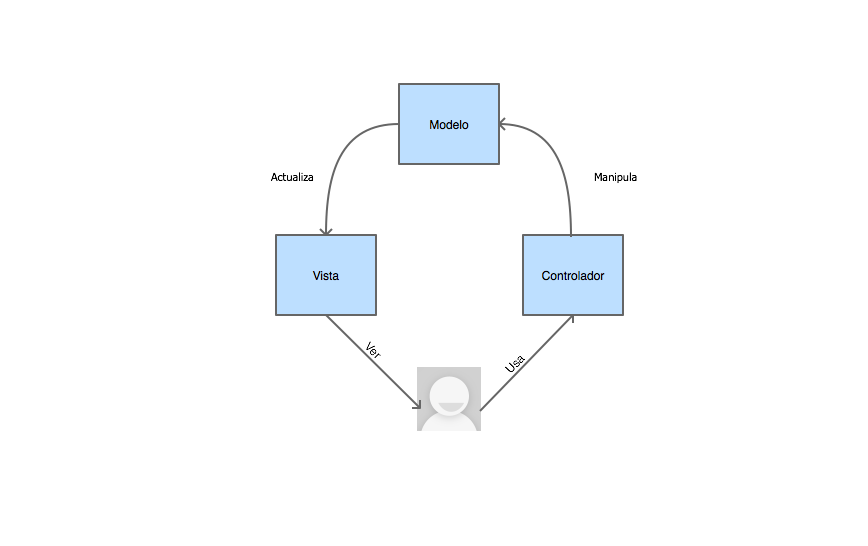
\includegraphics[scale=0.5]{imagenes/mvc.png}
\caption{Diagrama MVC}
\label{logo_mvc}
\end{center}
\end{figure}

\vspace{5 mm}

Crear una aplicación web basada en la arquitectura MVC nos ofrece ciertas ventajas. Por ejemplo, se puede dividir la lógica del negocio del diseño del sistema, haciendo el proyecto más escalable. Otra ventaja, es la existencia  de muchos frameworks basados en MVC como Laravel o Yii Framework, que permiten facilitar el trabajo de los desarrolladores. La implementación de URLs amigables, el control del uso de la memoria caché o el control de los recursos del servidor son tres de las principales ventajas de usar un framework MVC.


\section{Software}

Para diseñar una interfaz de usuario real, en la que poder basarme para luego representarla mediante HTML y CSS he utilizado diversos programas de diseño web.

\begin{itemize}

\item \textbf{Sketch}: Sketch es una aplicación de diseño vectorial, que te permite diseñar interfaces para aplicaciones móviles o web de una manera sencilla y con una gran potencia.
\item \textbf{Illustrator}: Esta herramienta de adobe tan famosa, te permite el diseño de logotipos de forma vectorial,
\item \textbf{Spectrum}: Programa sencillo que te permite crear paletas de colores, de forma que puedas seleccionar colores complementarios o de gama monocromática y utilizarlos para la interfaz de la aplicación.

\end{itemize}

\section{Tecnologías}

Para la realización de la aplicación web, se ha llevado a cabo un análisis de las tecnologías disponibles, y se han seleccionado las que mejor se adaptaban a las necesidades del proyecto.

\subsection{Front-End(Cliente)}

Las dos principales e indispensables tecnologías que se usan para la parte del cliente son el lenguaje de etiquetas HTML5 y las hojas de etilos CSS3. Estas son dos de las tecnologías fundamentales en las que se basa el desarrollo web.

 \vspace{5 mm}

 Con la finalidad de conseguir una apariencia cuidada e intuitiva del sitio web, sin la necesidad de crear las hojas de estilos propias, se planteó la idea de usar el framework Bootstrap. Finalmente debido al objetivo de personalizar al máximo la apariencia de la web, se descartó Bootstra y se optó por añadir clases propias mediante css.

\vspace{5 mm}

Para maquetar el sitio web con Css3 de forma más rápida y refactorizable utilizo \textbf{Sass}. Sass es un lenguaje de preprocesado de Css, que te permite escribir Css de forma más cómoda, permitiendote declarar variables,mixins, herencia de clases, etc. Hay diversas formas de utilizar Sass en tu proyecto. Mediante un programa como Prepros, mediante un automatizador de tareas como Grunt, o mediante un terminal con los comandos de Sass. Para el proyecto yo he optado usar el terminal para ejecutar Sass, ya que su ejecución es mucho más ligera y consume menos RAM que con programas como Prepros. Para que empezar a usar Sass en el proyecto, dentro de nuestra carpeta padre donde se encuentre el css, se crea una carpeta sass donde se incluirán todos los ficheros .scss. Con el terminal situado en la carpeta padre escribimos sass --watch sass(nombre de la carpeta donde se encuentran los ficheros .scss). Al compilarlo, nos generará un fichero style.css que será el estilo a usar.

\vspace{5 mm}

Para añadir el dinamismo a la web, se ha optado por utilizar un framework de Javascript como \textbf{JQuery} que permite simplificar la manera de interactuar con los documentos HTML, manipular el DOM, desarrollar animaciones y agregar peticiones AJAX. Además de que JQuery es software libre.

\vspace{5 mm}

Como última tecnología Front-End se utiliza la API de Google Maps, indispensable para el sitio web ya que la principal proposición de valor de la aplicación es la geolocalización de recetas, y para su representación necesitamos la API de Google.


\subsection{Back-End(Servidor)}

Después de barajar diversos lenguajes para desarrollar el back-end de la aplicación, finalmente me decanté por PHP. Además de ser el lenguaje más utlizado para el desarrollo web, es uno de los lenguajes más potentes y flexibles, pudiendo ser utilizado en la mayoría de los servidores web y sistemas operativos. Además PHP esta publicado bajo licencia de software libre, por lo que no supone ningun coste.


\vspace{5 mm}

Para montar la arquitectura MVC en la aplicación, utilizo el framwework Laravel. Laravel agiliza el desarrollo de las aplicaciones web, permitiendo multitud de funcionalidades. Con este framework, desarrollado de forma elegante y simple se evita la creación de código espagueti, faciltando su refactorización y/o su modificación. Algunas de las carácterísticas de Laravel: 


\begin{itemize}

\item \textbf{Plantillas}: Laravel utiliza platillas Blade. Blade permite tener un sitema de vistas modular de forma que se tenga que repetir la menor cantidad de código. Para ello se genera una plantilla base o layout, que es donde se representa la estructura de la web y se volcará el contenido para cada página. Mediante la directiva include(nombre\_template), se podrá incluir una vista parcial de contenido HTML, esta directiva se utiliza para contenido que no cambia por ejemplo para incluir la cabecera o el footer de la aplicación. Luego mediante la sentencia yield(nombre\_template) permitiremos crear una futura sección en el HTML que se definirá en las vistas que son heredadas de este template. Mediante la sentencia extends(nombre\_template) le diremos a Laravel que vistas se van a usar como futuras secciones. Con estas sentencias se conseguirá volcar el contenido especifíco para cada página de la web duplicando el menor numero de codigo HTML y de forma más modular.

\item \textbf{ORM}: Es una implementación de registro activo para trabajar con la base de datos de forma que cada tabla de la base de datos tiene un Modelo correspondiente asociado con el mismo nombre. Esta implementación te permite también métodos predefinidos para llamar a la base de datos como save(),create(),get(),find().

\item \textbf{Caché}: Laravel, cuenta con un robusto sistema de caché, el cual se puede ajustar, para que se produzca una carga rápida de la web y generar una mejor experiencia al usuario.

\item \textbf{MiddleWare}: Usa HTTP Middleware, que proporcionan un correcto mecanismo para filtrar las peticiones en la aplicación. Un ejemplo de middleware que incluye laravel, es el usado para verificar si el usuario esta autenticado en la aplicación.

\end{itemize}

\vspace{5 mm}

Para la base de datos, se utiliza el sistema de gestión relacional MySQL, ya que es uno de los sistemas más utilizados y con mayor documentación para el desarrollo web. Además, de la perfecta integración con Laravel.

\section{Modelo de Datos}

Como se ha comentado en el apartado anterior, el modelo de datos elegido para almacenar la información es el modelo relacional MySQL. El modelo relacional se fundamenta en el uso de relaciones, estas relaciones se pueden considerar como un conjunto de datos. Para mostrar una forma más visual esas relaciones se conceptualizan en forma de tablas, que estan formadas por registros y campos. En la figura \ref{tablas_bd} se representa mediante un modelo entidad-relacion los conjuntos de datos para la aplicación. Todas las tablas continene un campo Id que es el identificador de cada tabla(clave primaria) y tienen la clausula de auto-incremento por lo que cada vez que se agregue una fila, MySQL nos generará otro identificador incrementandolo en 1 valor.

\begin{figure}
\begin{center}
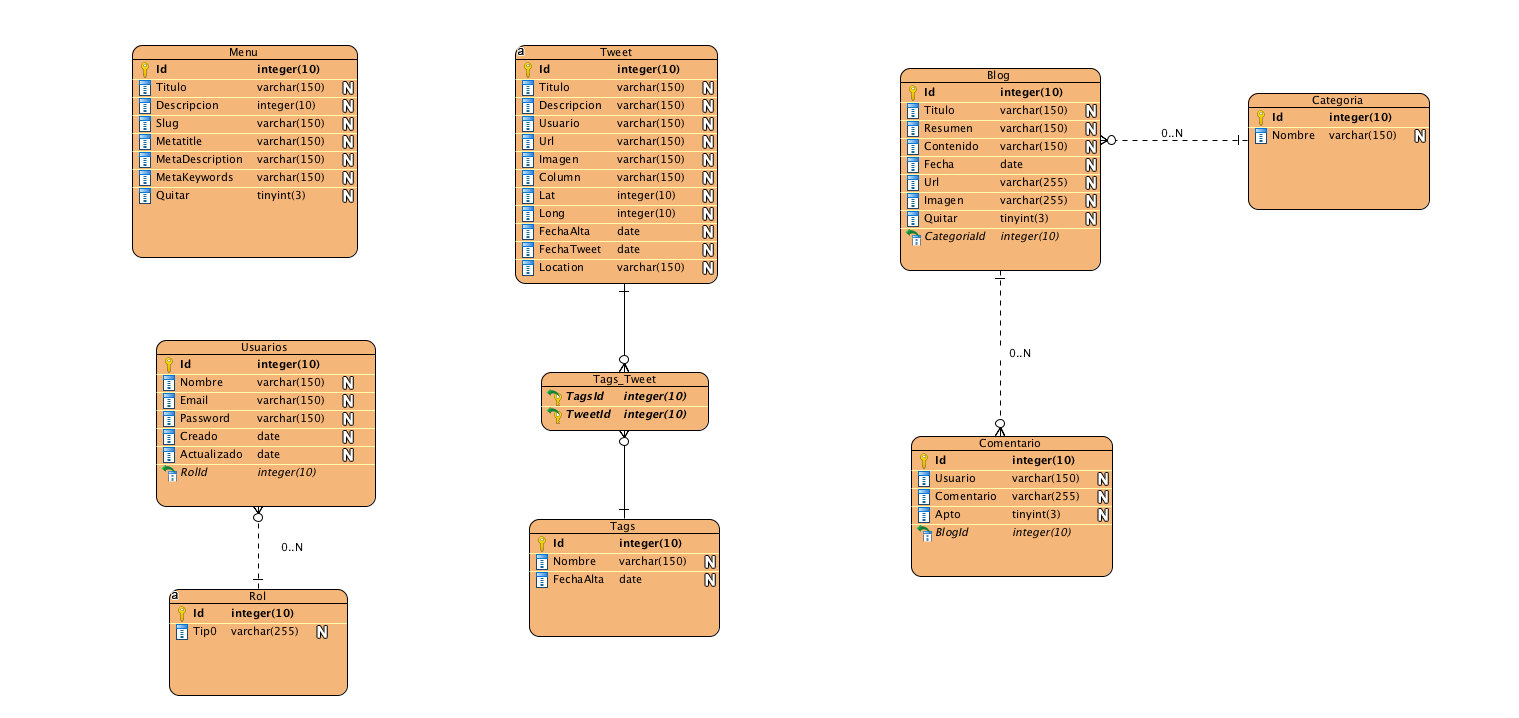
\includegraphics[width=1.0\textwidth]{imagenes/E-R.png}
\caption{Conjunto de tablas}
\label{tablas_bd}
\end{center}
\end{figure}

\begin{figure}
\begin{center}
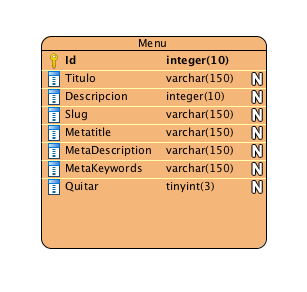
\includegraphics[scale=0.7]{imagenes/menu.png}
\caption{Tabla del menú}
\label{menu_bd}
\end{center}
\end{figure}

\begin{figure}
\begin{center}
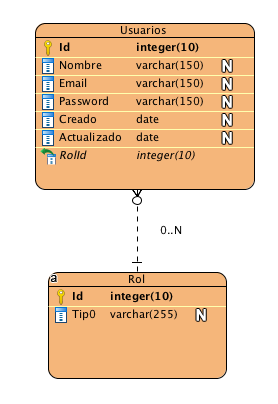
\includegraphics[scale=0.7]{imagenes/Usuarios.png}
\caption{}
\label{users_bd}
\end{center}
\end{figure}

\begin{figure}
\begin{center}
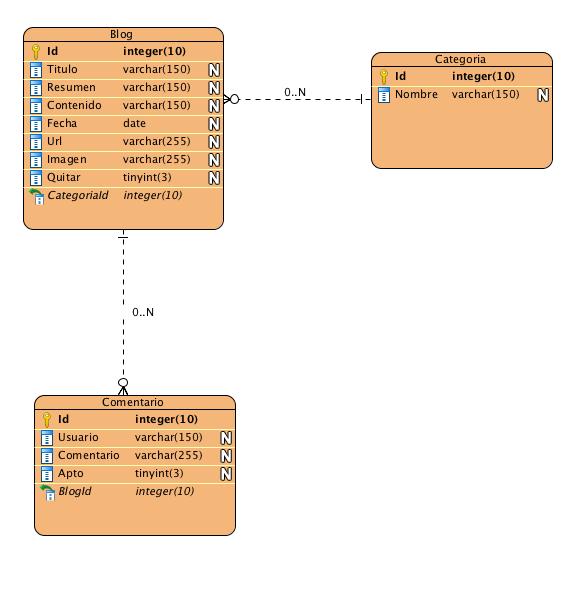
\includegraphics[scale=0.7]{imagenes/blog.png}
\caption{Tablas para el blog}
\label{blog_bd}
\end{center}
\end{figure}

\begin{figure}
\begin{center}
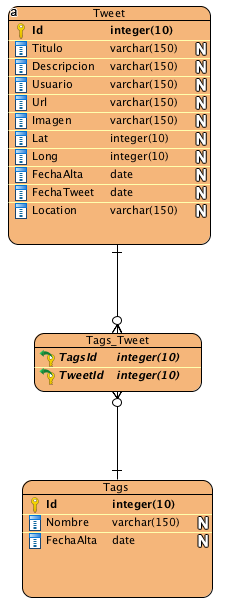
\includegraphics[scale=0.7]{imagenes/map.png}
\caption{Tablas para el mapa}
\label{map_bd}
\end{center}
\end{figure}


\vspace{5 mm}

La primera tabla, y más básica es la tabla de Menus, en ella encontramos todos los datos correspondientes al menu de navegación de la aplicación,esta tabla esta pensada para que el menú sea más dinamico y se pueda gestionar de forma más fácil sin modificar código. COmo se observa en la figura \ref{menu_bd}, la tabla de Menú se compone de los siguientes elementos:

\begin{itemize}

\item \textbf{Titulo}: Este es el titulo del menú, y el que aparecerá en la web en la navegación.
\item \textbf{Descripcion}: Campo para añadir texto introductorio, acerca de la sección.
\item \textbf{Slug}: El slug corresponde al trozo de la url que aparecerá para esa sección de la web en la aplicación.
\item \textbf{Campos de MetaAtributos}: MetaKeywords,MetaDescription,MetaTitle, los metas para cada sección del menú. Estos campos son importantes para un buen posicionamiento SEO.
\item \textbf{Quitar}: Campo de tipo tinyint, que nos permite dejar de mostrar un elemento del menú sin tener que borrar la fila. Por defecto el campo quitar esta a 0 y por tanto mostrará el elemento, en el caso de no se quiera visualizar, se cambia el valor a 1 y ese elemento ya no se muestra en el menu.

\end{itemize}

\vspace{5 mm}

En la figura \ref{users_bd}, se muestra la tabla de Usuarios y su relacion con los Roles de la aplicación. Se pretendía que un usuario tuviera un único rol y que un rol pudiera ser adoptado por muchos usuarios. Para representar esa relación se añade un clave ajena en la tabla usuarios generando una relacion uno a muchos y así permitiendonos cumplir las condiciones dictadas previamente.Para la tabla de Usuarios, se generan los siguientes campos:

\begin{itemize}

\item \textbf{Nombre}: Nombre del usuario, que se muestra en la web.
\item \textbf{Email}: Correo electrónico, del usuario. Tanto este campo como el nombre sirven de login para el usuario.
\item \textbf{Password}: Contraseña del usuario. En la base de datos se guarda un hash de la contraseña para mayor seguridad.
\item \textbf{Creado}: Campo de fecha con la creación del usuario.
\item \textbf{Actualizado}: Campo de fecha con la actualización del usuario.
\item \textbf{RolId}: Clave ajena a la tabla de Rol, contiene el Id del Rol.

\end{itemize}

\vspace{5 mm}

La tabla de Rol únicamente contiene el campo identificador y el tipo que hace referencia al nombre del rol.

\vspace{5 mm}

Para la página del Blog \ref{blog_bd} tenemos el esquema relacional con tres tablas: Blog,Categoría y Comentario. Cada fila de la tabla pertenece a una noticia del blog de la aplicación, cada noticia puede tener uno o más comentarios y ese comentario podrá aparecer solo en una noticia. Por tanto para cumplir esas condiciones se generan dos tablas(Blog y Comentario) con una relación uno a muchos. Las noticias pueden tener categorías, en el caso de la aplicación una noticía puede pertenecer a una categoría o ninguna, por tanto se añade una relación muchos a uno de la tabla Categoría a Blog. Las tuplas para la tabla de Blog son las siguientes:


\begin{itemize}

\item \textbf{Título}: Título de la noticia.
\item \textbf{Resumen}: Campo de texto para mostrar un resumen en el listado de noticias.
\item \textbf{Contenido}: Contenido de la noticia.
\item \textbf{Fecha}: Campo de Fecha con la creación de la noticia.
\item \textbf{Url}: Url amigable que aparece en la ruta de la noticia.
\item \textbf{Imagen}: Campo de texto para la imagen principal de la noticia.
\item \textbf{Quitar}: Campo quitar, para poder dejar de visualizar la noticia sin necesidad de borrarla de la base de datos.
\item \textbf{CategoríaId}: Clave ajena. Id de la categoría a la que pertenece la noticia.

\end{itemize}

\vspace{5 mm}

Tuplas para la tabla de comentarios:

\begin{itemize}

\item \textbf{Usuario}: Usuario que comenta la noticia.
\item \textbf{Comentario}: Campo de texto con el comentario sobre la noticia.
\item \textbf{Apto}: Campo para moderar el comentario y que sea valido para mostrar. Por defecto vale 1, no se muestra, cuando se cambia a cero se valida y se muestra.
\item \textbf{BlogId}: Clave ajena con el Id de la noticia al que pertence el comentario.


\end{itemize}

\vspace{5 mm}

Para el mapa de tweets se generan tres tablas(figura \ref{map_bd}). La principal es la tabla Tweet, donde se almacenan todos los tweets que se van a mostrar en el mapa. Los campos son los siguientes:


\begin{itemize}

\item \textbf{Título}: Título del tweet.
\item \textbf{Descripción}: Campo de texto que contiene el tweet.
\item \textbf{Usuario}: Usuario que ha escrito el tweet
\item \textbf{Url}: Enlace que se encuentra en el tweet y que te lleva a una página externa.
\item \textbf{Imagen}: Imagen del tweet.
\item \textbf{Lat}: Coordenada de latitud en el mapa.
\item \textbf{Long}: Coordenada de longitud en el mapa.
\item \textbf{FechaAlta}: Fecha de registro del tweet.
\item \textbf{FechaTweet}: Fecha de creación del tweet.
\item \textbf{Location}: Campo que guarda una localización.

\end{itemize}


\vspace{5 mm}


Para clasificar el contenido de los tweets, se crea la tabla Tags, que son los distintas clases en las que se pueden clasificar los tweets. Los campos para esta tabla son, el nombre de la etiqueta y la fecha de registro de la misma.

\vspace{5 mm}

Según como esta especificado, un tweet puede tener uno o más tags, y pueden pertenecer varios tweets a un tag. Por tanto es una relación muchos a muchos, para cumplir esta relación se crea una tabla adicional(Tag\_Tweets), que contiene los identificadores(es decir las claves primarias) de las dos tablas relacionadas(Tweet y Tag).









